\documentclass[12pt,a4paper]{article}
\usepackage[utf8]{inputenc}
\usepackage{lmodern}
\usepackage{amsmath, amsfonts, amssymb} % (\dfrac)
\usepackage{graphicx}

\begin{document}
    \textbf{INSERIR FIGURAS}
    
    \begin{enumerate}
        \item A imagem a seguir representa a utilização do MATLAB no estudo de sinais:
        
        \begin{figure}[htb]
            \centering
            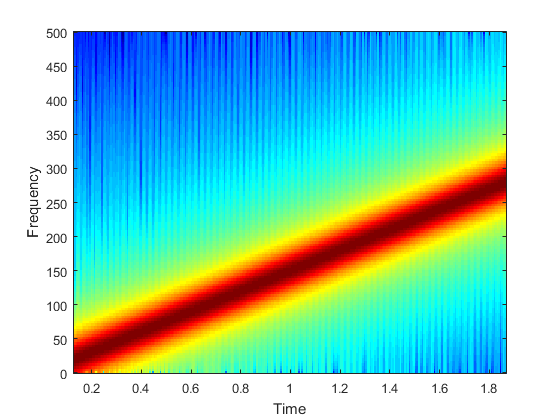
\includegraphics[scale=1]{sinal.png}
            \caption{Frequência em função do tempo}
            \label{fig:sinal}
        \end{figure}
    \end{enumerate}

    A Figura \ref{fig:sinal} contém um sinal arbitrário gerado pelo MATLAB. 
    
    
    
\end{document}
